\begin{adjustbox}{max width=\textwidth, max totalheight=0.6\textheight, center}
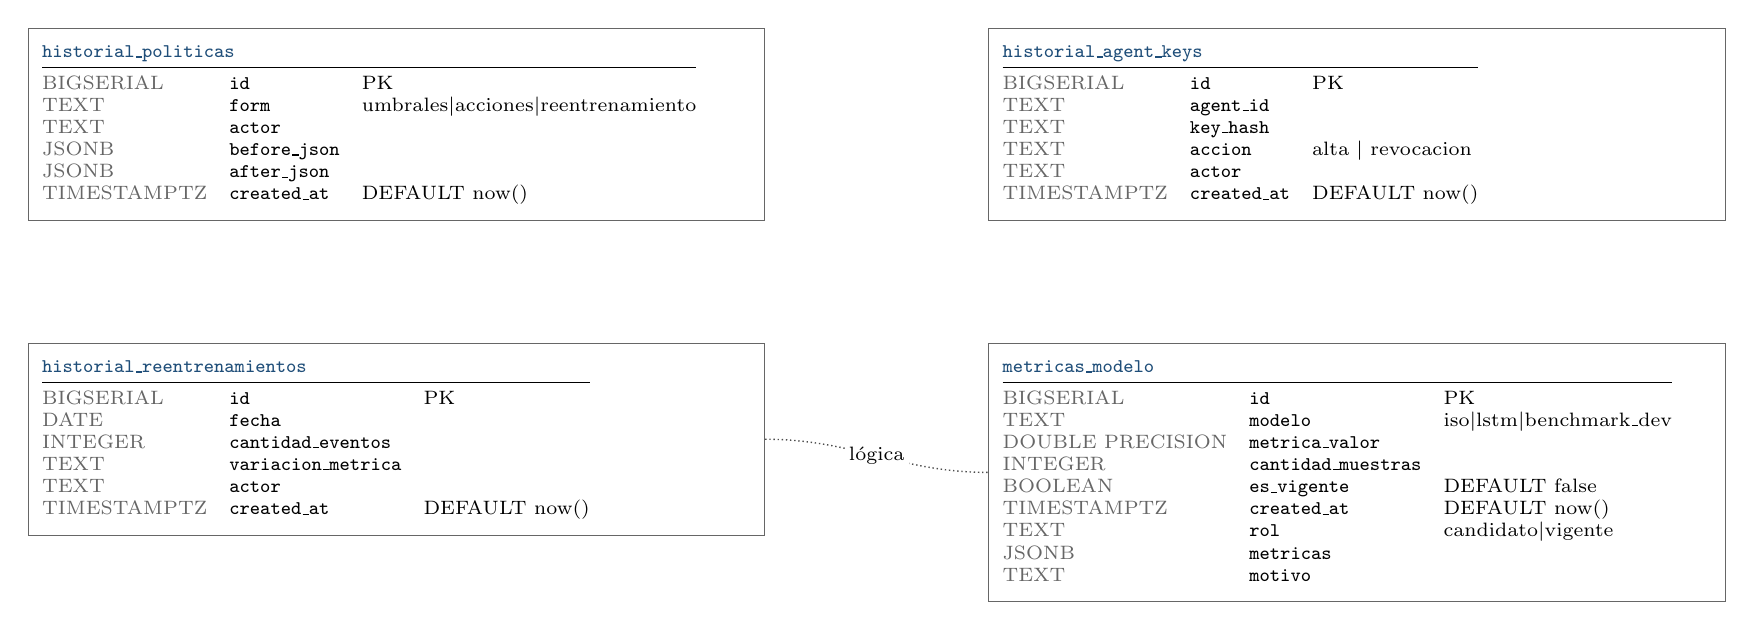
\begin{tikzpicture}[x=1cm, y=1cm]
% Estilos comunes de las figuras TikZ (despliegue y modelo relacional).
\definecolor{acento}{HTML}{1F4E79}
\hyphenpenalty=10000 \exhyphenpenalty=10000
\tikzset{
	caja/.style={draw=black!60, line width=0.4pt, fill=white, rounded corners=1pt, align=center, font=\footnotesize, inner sep=4pt, minimum height=0.9cm, text width=3.2cm},
	cajaacento/.style={caja, draw=acento, line width=0.7pt},
	opc/.style={caja, dashed, draw=black!55},
	almacen/.style={draw=black!60, line width=0.4pt, fill=black!6, cylinder, shape border rotate=90, aspect=0.22, align=center, font=\footnotesize, inner sep=3pt, minimum height=1.5cm, text width=2.6cm},
	zona/.style={draw=black!45, line width=0.4pt, fill=black!3, rounded corners=2pt, inner sep=8pt},
	zonaint/.style={draw=black!45, line width=0.4pt, fill=white, rounded corners=2pt, inner sep=7pt},
	flecha/.style={-{Stealth[length=5pt,width=4pt]}, line width=0.5pt, draw=black!70},
	rotulo/.style={font=\scriptsize, fill=white, inner sep=1.5pt},
	titulo/.style={font=\footnotesize\bfseries, text=black!75, anchor=south west},
}

\tikzset{tabla/.style={draw=black!60, line width=0.4pt, fill=white, inner sep=5pt, anchor=north west, font=\scriptsize, text width=9.0cm, align=left}}
\node[tabla] (po) at (0,0) {%
\begin{tabular}{@{}l@{\hspace{8pt}}l@{\hspace{8pt}}l@{}}
\multicolumn{3}{@{}l@{}}{\textcolor{acento}{\textbf{\texttt{historial\_politicas}}}} \\[1pt]
\hline
\noalign{\vskip 2pt}
\textcolor{black!60}{BIGSERIAL} & \texttt{id} & PK \\
\textcolor{black!60}{TEXT} & \texttt{form} & umbrales\textbar{}acciones\textbar{}reentrenamiento \\
\textcolor{black!60}{TEXT} & \texttt{actor} &  \\
\textcolor{black!60}{JSONB} & \texttt{before\_json} &  \\
\textcolor{black!60}{JSONB} & \texttt{after\_json} &  \\
\textcolor{black!60}{TIMESTAMPTZ} & \texttt{created\_at} & DEFAULT now() \\
\end{tabular}};
\node[tabla] (re) at (0,-4.0) {%
\begin{tabular}{@{}l@{\hspace{8pt}}l@{\hspace{8pt}}l@{}}
\multicolumn{3}{@{}l@{}}{\textcolor{acento}{\textbf{\texttt{historial\_reentrenamientos}}}} \\[1pt]
\hline
\noalign{\vskip 2pt}
\textcolor{black!60}{BIGSERIAL} & \texttt{id} & PK \\
\textcolor{black!60}{DATE} & \texttt{fecha} &  \\
\textcolor{black!60}{INTEGER} & \texttt{cantidad\_eventos} &  \\
\textcolor{black!60}{TEXT} & \texttt{variacion\_metrica} &  \\
\textcolor{black!60}{TEXT} & \texttt{actor} &  \\
\textcolor{black!60}{TIMESTAMPTZ} & \texttt{created\_at} & DEFAULT now() \\
\end{tabular}};
\node[tabla] (ak) at (12.2,0) {%
\begin{tabular}{@{}l@{\hspace{8pt}}l@{\hspace{8pt}}l@{}}
\multicolumn{3}{@{}l@{}}{\textcolor{acento}{\textbf{\texttt{historial\_agent\_keys}}}} \\[1pt]
\hline
\noalign{\vskip 2pt}
\textcolor{black!60}{BIGSERIAL} & \texttt{id} & PK \\
\textcolor{black!60}{TEXT} & \texttt{agent\_id} &  \\
\textcolor{black!60}{TEXT} & \texttt{key\_hash} &  \\
\textcolor{black!60}{TEXT} & \texttt{accion} & alta \textbar{} revocacion \\
\textcolor{black!60}{TEXT} & \texttt{actor} &  \\
\textcolor{black!60}{TIMESTAMPTZ} & \texttt{created\_at} & DEFAULT now() \\
\end{tabular}};
\node[tabla] (me) at (12.2,-4.0) {%
\begin{tabular}{@{}l@{\hspace{8pt}}l@{\hspace{8pt}}l@{}}
\multicolumn{3}{@{}l@{}}{\textcolor{acento}{\textbf{\texttt{metricas\_modelo}}}} \\[1pt]
\hline
\noalign{\vskip 2pt}
\textcolor{black!60}{BIGSERIAL} & \texttt{id} & PK \\
\textcolor{black!60}{TEXT} & \texttt{modelo} & iso\textbar{}lstm\textbar{}benchmark\_dev \\
\textcolor{black!60}{DOUBLE PRECISION} & \texttt{metrica\_valor} &  \\
\textcolor{black!60}{INTEGER} & \texttt{cantidad\_muestras} &  \\
\textcolor{black!60}{BOOLEAN} & \texttt{es\_vigente} & DEFAULT false \\
\textcolor{black!60}{TIMESTAMPTZ} & \texttt{created\_at} & DEFAULT now() \\
\textcolor{black!60}{TEXT} & \texttt{rol} & candidato\textbar{}vigente \\
\textcolor{black!60}{JSONB} & \texttt{metricas} &  \\
\textcolor{black!60}{TEXT} & \texttt{motivo} &  \\
\end{tabular}};
\draw[densely dotted, line width=0.5pt, draw=black!70] (re.east) to[out=0, in=180] node[rotulo, pos=0.5] {lógica} (me.west);
\end{tikzpicture}
\end{adjustbox}
